% This is samplepaper.tex, a sample chapter demonstrating the
% LLNCS macro package for Springer Computer Science proceedings;
% Version 2.20 of 2017/10/04
%
\documentclass{tlp} % \documentclass[runningheads]{llncs}

% \usepackage{graphicx}
\usepackage{amsmath}
% \usepackage{amssymb}
\usepackage{helvet,times,courier}
% \usepackage[inline]{enumitem}
% \usepackage{adjustbox}
% \usepackage{array}
% \newcolumntype{P}[1]{>{\centering\arraybackslash}p{#1}}
% \newcolumntype{M}[1]{>{\centering\arraybackslash}m{#1}}

\usepackage{tikz}
\usetikzlibrary{positioning,patterns}
\newlength{\scaledx}
\newlength{\scaledy}
\newcommand\SetScales{%
  \pgfextractx{\scaledx}{\pgfpointxy{1}{0}}%
  \pgfextracty{\scaledy}{\pgfpointxy{0}{1}}%
}

\usepackage{calc}
\newlength\listingnumberwidth
\setlength\listingnumberwidth{\widthof{\scriptsize 00} + 5pt}
% \setlength{\mathindent}{\listingnumberwidth}

\usepackage{listings}
\lstset{numberbychapter=false,numbers=left,numberblanklines=false,basicstyle=\ttfamily\small,numbersep=5pt,mathescape=true,escapeinside={\#(}{\#)},%xleftmargin=5ex,
xleftmargin=\listingnumberwidth,xrightmargin=3pt,captionpos=b,breaklines=false,frame=single}

\usepackage{multirow}
\usepackage{xspace}
\usepackage{url}

\usepackage{comment}
% Used for displaying a sample figure. If possible, figure files should
% be included in EPS format.
%
% If you use the hyperref package, please uncomment the following line
% to display URLs in blue roman font according to Springer's eBook style:
% \renewcommand\UrlFont{\color{blue}\rmfamily}

\newcommand{\clingo}{\emph{clingo}\xspace}
\newcommand{\clingodl}{\emph{clingo}[DL]\xspace}
\newcommand{\figspace}{\vspace{-1ex}}

\makeatletter
\def\fcapsize@figure{\normalfont\normalsize\rmfamily}
\def\fcapstyle@figure{\normalfont\normalsize\itshape}
\makeatother

\begin{document}

\lefttitle{Mohammed M.\ S.\ El-Kholany, Martin Gebser, Konstantin Schekotihin}

\jnlPage{1}{8}
\jnlDoiYr{2021}
\doival{10.1017/xxxxx}
%
\title{Problem Decomposition and Multi-shot ASP Solving for Job-shop Scheduling%
% \thanks{This work was partially funded by
% KWF project 28472,
% cms electronics GmbH,
% FunderMax GmbH,
% Hirsch Armbänder GmbH,
% incubed IT GmbH,
% Infineon Technologies Austria AG,
% Isovolta AG,
% Kostwein Holding GmbH, and
% Privatstiftung Kärntner Sparkasse.}%
}
%
%\titlerunning{Abbreviated paper title}
% If the paper title is too long for the running head, you can set
% an abbreviated paper title here
%
% \author{Mohammed M. S. El-Kholany\inst{1}\orcidID{0000-0002-1088-2081} \and
% Martin Gebser\inst{1,2}\orcidID{0000-0002-8010-4752} \and
% Konstantin Schekotihin\inst{1}\orcidID{0000-0002-0286-0958}}
% %
% \authorrunning{M. El-Kholany et al.}
% % First names are abbreviated in the running head.
% % If there are more than two authors, 'et al.' is used.
% %
% \institute{Alpen-Adria-Universität Klagenfurt, Klagenfurt, Austria 
% \email{\{mohammed.el-kholany, martin.gebser and konstantin.schekotihin\}@aau.at}\\
% %\url{http://www.springer.com/gp/computer-science/lncs} \and
% Technische Universität Graz, Graz, Austria\\
% \email{mgebser@ist.tugraz.at}}
\begin{authgrp}
\author{\sn{Mohammed M.\ S.} \gn{El-Kholany}} % \inst{1}\orcidID{0000-0002-1088-2081} \and
\affiliation{University of Klagenfurt, Austria \and Cairo University, Egypt}
\author{\sn{Martin} \gn{Gebser}} % \inst{1,2}\orcidID{0000-0002-8010-4752} \and
\affiliation{University of Klagenfurt, Austria \and Graz University of Technology, Austria}
\author{\sn{Konstantin} \gn{Schekotihin}} % \inst{1}\orcidID{0000-0002-0286-0958}
\affiliation{University of Klagenfurt, Austria}
\end{authgrp}

\history{\sub{xx xx xxxx;} \rev{xx xx xxxx;} \acc{xx xx xxxx}}

\maketitle              % typeset the header of the contribution
%
\begin{abstract}
Scheduling methods are important for effective production and logistics management, where tasks need to be allocated and performed by limited resources.
In particular, the Job-shop Scheduling Problem (JSP) is a well-known and challenging
combinatorial optimization problem in which tasks sharing a machine are to be arranged
in sequence such that encompassing jobs can be completed as early as possible.
Given that already moderately sized JSP instances can turn out as highly combinatorial,
so that neither optimal schedules nor the runtime to termination of complete optimization methods
is known, efficient approaches to approximate good-quality schedules are of interest.
In this paper, we propose problem decomposition into time windows whose operations
can be successively scheduled and optimized by means of multi-shot ASP solving.
From a computational perspective, decomposition aims to split highly complex scheduling tasks into better manageable subproblems with a balanced number of 
operations, so that good-quality or even optimal partial solutions can be
reliably found in a small fraction of runtime.
Regarding the feasibility and quality of solutions, problem decomposition must
respect the precedence of operations within their jobs, and partial schedules
optimized by time windows should yield better global solutions than obtainable
in similar runtime on the full problem.
We devise and investigate a variety of decomposition strategies in terms of the number and size of time windows as well as heuristics for choosing their operations.
Moreover, we incorporate time window overlapping and compression techniques
into the iterative scheduling process in order to counteract limitations of window-wise optimization restricted to partial schedules.
Our experiments on JSP benchmark sets of several sizes show that
successive optimization by multi-shot ASP solving leads to substantially better schedules within the runtime limit than global optimization on the full problem,
where the gap increases with the number of operations to schedule.
%
% This paper applied a decomposition approach that splits the problem into a pre-defined set of small problems called Time Windows (TWs) and solves each separately in sequential order. Our proposed model is split into two main phases for solving the (JSP). The decomposition phase assigns each operation to a particular TW while satisfying the precedence constraint. The second phase is the scheduling phase, in which the model starts to optimize the first TW and continues until finishing the last TW. We built our model using Answer Set Programming (ASP). A Multi-shot solving paradigm is used to deal with the decomposition approach and differenc logic to handle the constraints. To evaluate the proposed work, we tested our model on a set of benchmark instances with different sizes and the results showed that the multi-shot solving is better than the single-shot when the number of operations increases. 
% \keywords{Job-shop Scheduling Problem  \and Answer Set Programming \and Decomposition.}
\end{abstract}
%
\begin{keywords}
Job-shop Scheduling Problem, Answer Set Programming, Problem Decomposition
\end{keywords}
%
%
\section{Introduction}
% In today's competitive markets, manufacturers have to respond quickly to orders and meet shipping dates committed to the customers. This requires the ability to schedule production activities to use the available scarce resources efficiently. Effective scheduling techniques are essential in complex manufacturing systems such as semiconductor manufacturing. In general, scheduling operations is one of the most critical issues in the planning and managing of the manufacturing processes\cite{uzsoy2000performance}.
Effective scheduling methods are essential for complex manufacturing and logistics systems,
where allocating and performing diverse tasks within resource capacity limits 
is one of the most critical challenges for production management \citep{uzsoy2000performance}.
The Job-shop Scheduling Problem (JSP) \citep{baker1974introduction,taillard1993benchmarks}
constitutes a well-known mathematical abstraction of industrial production scheduling in
which sequences of operations need to be processed by machines such that a given objective
like the makespan for completing all jobs or their tardiness w.r.t.\ deadlines is minimized.
Finding optimal JSP solutions, determined by a sequence of operations for each machine,
is an NP-hard combinatorial problem
\citep{garey1976complexity,lenstra1977complexity,liu2008prediction},
and optimal schedules as well as termination guarantees can be extremely challenging
or beyond reach 
of complete optimization methods already for moderately sized instances.
For example, it took about $20$ years to develop a search procedure able to find a
(provably) optimal solution for an instance called FT10 with $10$ jobs
\citep{adams1988shifting,zhang2010hybrid},
each consisting of a sequence of $10$ operations to be processed by $10$ machines. 

% One of the most challenging scheduling problems is the Jop-shop Scheduling Problem (JSP). A set of jobs needs to be processed on a set of machines while optimizing a performance indicator, minimizing makespan, the time needed to complete all the jobs, or tardiness, i.e., the summation of the delays in executing all jobs according to their deadlines. Each job has a set of consecutive operations; each operation requires exactly one machine; machines are continuously available and can process only one operation at a time. The main purpose is to determine the sequence of the operations on each machine to optimize a performance indicator. The JSP is an NP-complete combinatorial optimization problem where obtaining the optimal solution is challenging regardless of the problem scale\cite{garey1976complexity,lenstra1977complexity,liu2008prediction}. For instance, benchmark (FT10) consists of $10$ jobs and $10$ machines took researchers roughly $20$ years to find the optimal solution\cite{adams1988shifting,zhang2010hybrid}.

In real-world production scheduling, the number of operations to process can easily go
into tens of thousands \citep{coltep19a,kohakamo20a,kotakoscge21a}, which exceeds exact
optimization capacities even of state-of-the-art solvers for Answer Set Programming (ASP),
Mixed Integer Programming (MIP), or Constraint Programming (CP)
\citep{daneshamooz2021mathematical,francescutto2021solving,shi2021solving}.
Hence, more efficient approaches to approximate good-quality schedules 
instead of striving for optimal solutions have attracted wide research interest.
On the one hand, respective methods include greedy and local search techniques such as
dispatching rules \citep{blackstone1982state}, shifting bottleneck \citep{adams1988shifting} and
genetic algorithms \citep{pezzella2008genetic}.
On the other hand, problem decomposition strategies based on a
rolling horizon \citep{singer2001decomposition,liu2008prediction} or
bottleneck operations \citep{zhang2010hybrid,zhai2014decomposition} 
have been proposed to partition large-scale instances into better manageable subproblems,
where no single strategy strictly dominates \citep{ovacik2012decomposition}.

% In reality, the number of operations is reaching thousands of operations. Therefore, the exact methods Answer Set Programming (ASP), Constraint Programming and Branch and Bound cannot find the optimal solutions in a reasonable time\cite{daneshamooz2021mathematical,shi2021solving,francescutto2021solving}. Since the performance of the exact methods will be hardly satisfactory, several studies have presented one of the most effective methods for solving the JSP, which is decomposition \cite{zhang2010hybrid}. The decomposition aims to split the problem into a series of subproblems based on a particular decomposition policy and then solve each part separately and obtain the final solution by integrating all of these solutions. Several strategies have been proposed to decompose the JSP, and each varies according to the problem features. More specifically, there is no evidence that one of the introduced strategies is the best for solving all JSP(s) \cite{ovacik2012decomposition}. 

While decision versions of scheduling problems can be successfully modeled and
solved by an extension of ASP with Difference Logic (DL) constraints
\citep{gebser2016theory}, implemented by \clingodl on top of the
(multi-shot) ASP system \clingo \citep{gekakasc17a},
the optimization capacities of \clingodl come to their limits on moderately sized
yet highly combinatorial JSP instances \citep{elkgeb20a}, for some of which optimal solutions are so far unknown \citep{shysha18a}.
Successful application areas beyond JSP include 
industrial printing \citep{balduccini11a},
team-building \citep{rigralmaliiile12a},
shift design \citep{abseher2016shift},
course timetabling \citep{bainkaokscsotawa18a},
lab resource allocation \citep{francescutto2021solving},
and
medical treatment planning \citep{dogagrmamopo21a},
pointing out the general attractiveness of ASP for modeling and solving scheduling problems.

In this paper, we greatly extend our preliminary study \citep{elkgeb20a} 
on problem decomposition into time windows and successive schedule optimization
by means of multi-shot ASP modulo DL solving with \clingodl.
The goal of the decomposition is to split highly complex scheduling tasks into
balanced portions for which partial schedules of good quality can be reliably
found within tight runtime limits, and then be merged into a global solution of
significantly better quality than obtainable in similar runtime 
with single-shot optimization on the full problem.
In this process, problem decomposition must respect the precedence of operations
within their encompassing jobs to guarantee the feasibility of schedules, and as
a secondary objective, the order by time windows of operations sharing a machine should come close to the sequences of operations in (unknown) optimal schedules.
We address computational efficiency as well as solution quality by devising and investigating decomposition strategies regarding the size of
time windows and heuristics to choose their operations.

The contributions of our work going beyond the study in \citep{elkgeb20a} are:
\begin{itemize}
\item In addition to problem decomposition based on the earliest starting times
      of operations, we consider the most total work remaining criterion and
      refinements of both strategies by bottleneck machines.
      We encode static as well as dynamic decomposition variants, the latter taking
      partial schedules for operations of previous time windows into account, by stratified
      ASP programs (without DL constraints).
\item Considering that a decomposition into time windows may be incompatible with
      the optimal sequences of operations sharing a machine, we incorporate
      time window overlapping into the iterative scheduling process to
      offer a chance for revising "decomposition mistakes".
      Moreover, as the makespan objective we apply for the optimization of
      (partial) schedules tolerates unnecessary idle times of machines as long as
      they do not yield a greater scheduling horizon,
      we devise a stratified ASP encoding to postprocess and compress partial
      schedules by reassigning operations to earlier idle slots available on their machines.
\item We experimentally evaluate decomposition strategies varying the number of
      operations per time window as well as multi-shot ASP solving
      augmented with overlapping and compression techniques
      on JSP benchmark sets of several sizes.
      In particular, our experiments demonstrate that successive optimization
      by multi-shot ASP solving leads to substantially better schedules within
      tight runtime limits than global optimization on the full problem,
      where the gap increases with the number of operations to schedule.
\end{itemize}

% In this study, we aim to introduce a new decomposition strategy for solving the JSP. Our study proposes a new policy to efficiently divide the problem into subproblems, aiming to reach a near-optimal solution. Then each part is solved using an ASP scheduler-based, and the solutions are integrated to obtain the solution of the whole problem. We develop and implement our model using ASP, which is considered as one of the most popular paradigms for knowledge representation and reasoning, especially in combinatorial optimization problems \cite{abseher2016shift}. 

The rest of this 
paper is organized as follows.
Section~\ref{sec:preliminaries} briefly introduces ASP along with the relevant
extensions of multi-shot solving and DL constraints.
In Section~\ref{sec:problem}, we present our successive optimization approach
and detail the ASP programs encoding problem decomposition or iterative scheduling by
time windows, respectively.
Section~\ref{sec:experiments} provides experimental results on JSP benchmark sets, % of several sizes,
assessing different decomposition strategies as well as the impact of overlapping and
compression techniques.
Conclusions and future work are discussed in Section~\ref{sec:conclusions}.  
% The following section shows the most related work and which decomposition techniques have been introduced in the past, followed by the problem formulation section illustrates the problem in detail. Section $4$ presents our proposed model, which shows the decomposition techniques we used and describes one in more detail. In addition, we present the schedule model using Answer Set Programming. Our model is tested by performing extensive experiments on a set of benchmark instances in Section $5$. Section $6$ summarizes this work and provides some ideas to extend the current work.

% \section{Literature Review}
% This section will review some of the work that has applied the decomposition approach for solving scheduling problems. As mentioned in the previous section, no particular decomposition method has proved its efficiency in solving all scheduling problems. However, many articles have introduced efficient decomposition methods for solving particular scheduling problems with specific features. The decomposition idea for solving JSP has been initially suggested by introducing a \textit{Shifting bottleneck} (SB) procedure which decomposes the problem into parts; each part contains only one machine \cite{adams1988shifting}. At each iteration, the bottleneck machine is determined from a set of unsequenced machines and then scheduled. Afterward, all the previously established sequences are locally reoptimized and iterate until all the machines have been sequenced. The idea of SB had been later improved by integrating an optimization algorithm for solving the one-machine problem with the delayed precedence constraints procedure \cite{balas1995one}.

% Another study investigated the performance of a new decomposition procedure based on SB in the Job-shop and flow shop with different levels of bottleneck machines. The computational experiments showed that the proposed method obtained better solutions in a shorter time than for the problems in which the machine's workload is identical. Other different methods have been developed to decompose the JSP. For instance, a rolling horizon heuristic has been presented \cite{singer2001decomposition} to solve a large-scale job shop. The authors have decomposed the problem and solve each independently while minimizing the total weighted tardiness. They tested their model on a set of benchmark instances, and the results showed that the proposed model is superior to large instances. 

% The rolling horizon procedure has been extended by constructing a prediction model to obtain the scheduling characteristics values, including the information of the bottleneck jobs. The obtained information aided in decomposing the problem efficiently. In addition, they have proposed a genetic algorithm to solve each sub-problem. In order to evaluate the performance of the proposed model, they performed numerical computational experiments that showed the effectiveness of the model \cite{liu2008prediction}. A decomposition-based hybrid optimization algorithm has been introduced for the JSP, where the total weighted tardiness is minimized. A Simulated Annealing is used to define subproblems iteratively and then is solved by a Genetic Algorithm. They have developed a fuzzy system that provides information about bottleneck jobs. This information is used to guide the process of subproblem-solving to promote the optimization efficiency \cite{zhang2010hybrid}. The numerical computational results showed that the proposed algorithm is effective for large-scale scheduling problems.

% A decomposition method based on bottleneck machines has been presented for solving the JSP. The proposed model decomposes the problems into subproblems and then detects the multi-bottleneck machines using a critical path method. The information of the bottleneck machines has been employed to improve the solution quality by splitting the operations into bottleneck operations and non-bottleneck operations, where the bottleneck operations are scheduled by the Genetic Algorithm and the non-bottleneck operations are scheduled by dispatching rules \cite{zhai2014decomposition}.

% From the literature, we can find that most of the related work focused on applying the decomposition approach while minimizing the total tardiness, and the number of work tackled large-scale instances to minimize the makespan is relatively low. This paper proposes different decomposition strategies for solving the JSP with larger instances using the ASP model while minimizing the makespan.

\section{Preliminaries}\label{sec:preliminaries}
\paragraph{Answer Set Programming (ASP)} is a declarative programming language for solving hard combinatorial optimization problems. ASP has become an established paradigm for knowledge representation and reasoning. ASP has proved its efficiency for solving the combinatorial optimization problem in different applications such as bioinformatics\cite{erdem2015generating,koponen2015optimizing}, databses\cite{caniupan2010consistency} and scheduling and industrial applications~\cite{dodaro2015allotment,dodaro2016combining,fabricius2020towards,dodaro2021operating}.

A logic program is a finite set of rules of the form 
\begin{equation}
	a_0 \gets a_1, \ldots, a_m, \sim a_{m+1}, \dots, \sim a_n
	\label{rule1}
\end{equation}
where $a_i$ is an atom for $0 \leq i \leq n$ and ``$\sim$''  is a default negation. If $n$ quals to $0$, then a rule \eqref{rule1} is a fact. If $a_0$ is omitted, the rule is an integrity constraint. An \emph{atom} is an expression of the form $p(t_1,\ldots,t_l)$, where $p$ is a predicate and $t_1,\ldots,t_l$ are \emph{terms}. Each term can be a variable or a constant. A \emph{literal} is either an atom or its negation. 
Given a rule $r$ of the form \eqref{rule1}, the set $H(r)=a_0$ denotes the \emph{head} atom and the set $B(r) = B^+(r) \cup B^-(r) = \{a_1,\dots,a_m\} \cup \{\sim a_{m+1}, \dots \sim a_n\}$ is the \emph{body} of $r$ where $B^+(r)$ and $B^+(r)$ represent the positive and negative body literals, respectively.
\paragraph{Multi-shot Solving:}
Multi-shot solving ASP allows solving logic programs dynamically in sequential order. This can be manipulated using APIs implementation via an imperative programming language. Such programming language is used to control the grounding and solving processes and allows the usage of external variables that could be set to $True$ or $False$ to control some logic rules. The main advantage of \emph{multi-shot} solving is to avoid the re-grounding and exploit conflicts learned over time.
%ASP is a paradigm that deals with continuously changing logic programs. In a single-shot approach, an ASP system takes a logic program, computes answer sets and exits. However, the idea of Multi-shot is to consider evolving grounding and solving processes. \emph{clingo} systems enhances the ASP declaritive language with control capacities. 
\paragraph{ASP Difference Logic:}
\emph{clingo}[DL] is an extension of the input language \emph{clingo} by theory atoms representing difference constraints \cite{gebser2016theory,janhunen2017clingo}. Difference constraints are defined by specific constraint atoms of the form $\text{\lstinline{&diff}}\{u-v\} \leq k$ where $u$ and $v$ are terms which are interpreted as integer variables and $k$ is an integer constant. \emph{clingo}[DL] provides the following extension of the normal form \eqref{rule1}: 
\begin{align*}
	\text{\lstinline{&diff}}\{u-v\} \leq k \gets a_1, \ldots, a_m, \sim a_{m+1}, \ldots, \sim a_n.
\end{align*}
 This rule shows that whenever the body is $True$ the inequality constraints must be satisfied.

\section{Multi-shot JSP Solving}\label{sec:problem}
This section describes our successive optimization approach to
JSP solving by means of multi-shot ASP with \clingodl.
We start with specifying the fact format for JSP instances,
then detail problem decomposition based on earliest starting times of operations,
present our ASP encoding with DL constraints for optimizing the makespan of partial schedules, and
finally outline the incorporation of time window overlapping and compression
into the iterative scheduling process.   
% The Job-shop Scheduling Problem (JSP) has been a complex and combinatorial optimization problem since the 1950s, and it was shown to be NP-hard. In the JSP, there are a set of jobs to be processed on a set of machines. The number of jobs is $n$, and the number of machines is $m$. Each job $J_i$ contains a chain $ O_{i,1}, O_{i,2},...,O_{i,m} $ of operations must be executed on an known order. The routings of the operations are deterministic and known a priori, as are the processing times of each operation on each machine. We consider here the problem of minimizing the total completion time (makespan). The task of the scheduling is to determine the starting time for each operation while optimizing the makespan. The basic assumptions are as follows:
%
% \begin{enumerate}
% 	\item The processing time of each operation is fixed.
% 	\item Machine breakdown preemption of the operations are not allowed.
% 	\item Each machine can process only one operation at a time.
% 	\item Each operation can be executed by only one machine.
% 	\item A machine cannot process more than one operation at a time.
% 	\item The jobs and the machines are available at time $0$.
% \end{enumerate}

\subsection{Problem Instance}\label{subsec:instance}
% ASP has been applied to solve different scheduling problems. For example, ASP is used to solve scheduling problems in the healthcare systems \cite{dodaro2017nurse,dodaro2019asp}. One of these studies aimed to assign nurses to shifts according to some constraints\cite{dodaro2017nurse}. In addition, ASP has been proposed to solve a train scheduling problem while minimizing the train delay\cite{abels2019train}. One of the limitations of ASP mentioned in these studies is the grounding issues while solving a large number of instances. One of the recent works has presented a multi-shot solving for scheduling problem \cite{francescutto2021solving}. This paper aims to use different decomposition methods to solve the JSP using ASP with Difference Logic. 
% 
% \paragraph{Problem Instances.} 
%
Each job in a JSP instance is a sequence of operations with associated
machines and processing times.
Corresponding facts for an example instance with three jobs and three
machines are displayed in Listing~\ref{prg:facts}.
An atom of the form
\lstinline{operation(}$j$\lstinline{,}$s$\lstinline{,}$m$\lstinline{,}$p$\lstinline{)}
denotes that the step~$s$ of job~$j$ needs to be processed by machine~$m$ for $p$ time units.
For example, the second operation of job~\lstinline{3} has a processing time of
\lstinline{3} time units on machine~\lstinline{1},
as specified by the fact
\lstinline{operation(3,}\linebreak[1]\lstinline{2,}\linebreak[1]\lstinline{1,3).}
The operation cannot be performed before the first operation of job~\lstinline{3}
is completed,
and its execution must not intersect with the first operation of job~\lstinline{1}
or the second operation of job~\lstinline{2},
which need to be processed by machine~\lstinline{1} as well.
That is, a schedule for the example instance must determine a sequence in which
to process the three mentioned operations on machine~\lstinline{1},
and likewise for operations sharing machine~\lstinline{2} or~\lstinline{3}, respectively.
%
% In order to encode the problem using ASP, we should define a set of predicates that represents the problem instances. For instance, the operations are encoded with the predicate \lstinline{operation/2} where the first variable denotes the job number and the second is the operation number, see lines \ref{prg:facts:ops:begin}-\ref{prg:facts:ops:end} in Listing \ref{prg:facts}. The time needed to finish an operation is represented by the predicate \lstinline{pro/3} in which the operation is determined by the first two terms and the third represents the processing time in lines \ref{prg:facts:pro:begin}-\ref{prg:facts:pro:end}. For the machine assignment, the predicate \lstinline{assign/3} shows that a particular operation is executed by a machine in lines \ref{prg:facts:mach:begin}-\ref{prg:facts:mach:end}. For instance, \emph{operation(1,1)} is processed by machine 2. 
\lstinputlisting[float=t,label=prg:facts,caption={Example JSP instance},linerange={1-3},numbers=none,xleftmargin=3pt]{listing/facts.lp}

Figure~\ref{fig:schedule} depicts an optimal schedule in terms of makespan,
i.e., the latest completion time of any job/operation,
for the JSP instance from Listing~\ref{prg:facts}.
The \textbf{J}-\textbf{S} pairs in horizontal bars indicated for the
machines~\lstinline{1}, \lstinline{2}, and~\lstinline{3} identify operations
by their job~\textbf{J} and step number~\textbf{S}.
For each machine, observe that the bars for operations it processes do not
intersect, so that the operations are performed in sequential order.
Moreover, operations belonging to the same job are scheduled one after the other.
For example,
the second operation of job~\lstinline{3} is only started after the
completion of the predecessor operation at time~$9$,
regardless of the availability of its machine~\lstinline{1}
from time~$3$ on.
As the precedence of operations within their jobs must be respected
and the sum of processing times for operations of job~\lstinline{3}
matches the makespan~$20$, it is impossible to reduce the scheduling
horizon any further,
which in turn means that the schedule shown in Figure~\ref{fig:schedule} is optimal.
%
\begin{figure}[t]
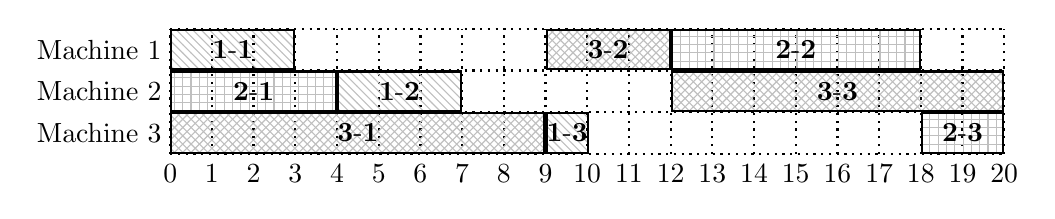
\begin{tikzpicture}[x=3.5ex,y=3.5ex,label distance=-1ex,thick]
\SetScales
\foreach \i in {1,...,3} {
  \node[label=left:Machine \i] at (0,3.5-\i) {};
}
\foreach \i in {0,...,20} {
  \draw[dotted] (\i,0) -- (\i,3) node [below] at (\i,0) {$\i$};
}
\foreach \i in {0,...,3} {
  \draw[dotted] (0,\i) -- (20,\i);
}
\node[minimum width=3\scaledx-0.05\scaledx,minimum height=1\scaledy-0.05\scaledy,inner sep=0,rectangle,draw,anchor=south west,pattern color=lightgray,pattern=north west lines] at (0,2) {\textbf{1}-\textbf{1}};
\node[minimum width=3\scaledx-0.05\scaledx,minimum height=1\scaledy-0.05\scaledy,inner sep=0,rectangle,draw,anchor=south west,pattern color=lightgray,pattern=crosshatch] at (9,2) {\textbf{3}-\textbf{2}};
\node[minimum width=6\scaledx-0.05\scaledx,minimum height=1\scaledy-0.05\scaledy,inner sep=0,rectangle,draw,anchor=south west,pattern color=lightgray,pattern=grid] at (12,2) {\textbf{2}-\textbf{2}};
\node[minimum width=4\scaledx-0.05\scaledx,minimum height=1\scaledy-0.05\scaledy,inner sep=0,rectangle,draw,anchor=south west,pattern color=lightgray,pattern=grid] at (0,1) {\textbf{2}-\textbf{1}};
\node[minimum width=3\scaledx-0.05\scaledx,minimum height=1\scaledy-0.05\scaledy,inner sep=0,rectangle,draw,anchor=south west,pattern color=lightgray,pattern=north west lines] at (4,1) {\textbf{1}-\textbf{2}};
\node[minimum width=8\scaledx-0.05\scaledx,minimum height=1\scaledy-0.05\scaledy,inner sep=0,rectangle,draw,anchor=south west,pattern color=lightgray,pattern=crosshatch] at (12,1) {\textbf{3}-\textbf{3}};
\node[minimum width=9\scaledx-0.05\scaledx,minimum height=1\scaledy-0.05\scaledy,inner sep=0,rectangle,draw,anchor=south west,pattern color=lightgray,pattern=crosshatch] at (0,0) {\textbf{3}-\textbf{1}};
\node[minimum width=1\scaledx-0.05\scaledx,minimum height=1\scaledy-0.05\scaledy,inner sep=0,rectangle,draw,anchor=south west,pattern color=lightgray,pattern=north west lines] at (9,0) {\textbf{1}-\textbf{3}};
\node[minimum width=2\scaledx-0.05\scaledx,minimum height=1\scaledy-0.05\scaledy,inner sep=0,rectangle,draw,anchor=south west,pattern color=lightgray,pattern=grid] at (18,0) {\textbf{2}-\textbf{3}};
\end{tikzpicture}
\figspace
\caption{Optimal schedule for example JSP instance\label{fig:schedule}}% in Listing~\ref{prg:facts}\label{fig:schedule}}
\end{figure}

\subsection{Problem Decomposition}\label{subsec:decomposition}
%
Since JSP instances are highly combinatorial and the ground representation size
can also become problematic for large real-world scheduling problems, achieving
scalability of complete optimization methods necessitates problem decomposition.
To this end, we consider strategies for partitioning the operations of JSP instances
into balanced time windows, which respect the operation precedence within jobs and
enable a successive extension of good-quality partial schedules to a global solution.
In the following, we first detail problem decomposition based on earliest starting
times of operations, and then outline further strategies that can be encoded
by stratified ASP programs as well.

\lstinputlisting[float=t,label=prg:decomposition,caption={Job-based EST decomposition encoding}]{listing/decomposition.lp}
%
Our encoding for \emph{Job-based Earliest Starting Time (EST)} decomposition
in Listing~\ref{prg:decomposition} takes a JSP instance specified by facts over
\lstinline{operation/4} as input.
In addition, a constant~\lstinline{n},
set to the default value~\lstinline{2} in line~\ref{prg:predeco:tw:begin},
determines the number of time windows into which the given operations
shall be split.
As we aim at time windows of (roughly) similar size,
the target number of operations per time window is in line~\ref{prg:predeco:optw:begin}
calculated by $\lceil \text{\lstinline{N}} / \text{\lstinline{n}}\rceil$,
where \lstinline{N} is the total number of operations.
For example, we obtain \lstinline{width(5)} for partitioning the nine operations
of the JSP instance in Listing~\ref{prg:facts} into two time windows.

The rules in lines~\ref{prg:assignment_process:est:begin} and~\ref{prg:assignment_process:est:end}
encode the EST calculation per operation of a job,
given by the sum of processing times for predecessor operations belonging to the same job.
This yields, e.g., 
\lstinline{est(3,1,9,0)},
\lstinline{est(3,2,3,9)}, and
\lstinline{est(3,3,8,12)}
for the three operations of job~\lstinline{3} in our example instance,
where the third argument of an atom over \lstinline{est/4} provides
the processing time and the fourth the earliest starting time of an operation.
Note that the obtained earliest starting times match the first feasible time
points for scheduling operations and do thus constitute an optimistic
estimation of when to process the operations.

With the earliest starting times of operations at hand,
the rule in lines \ref{prg:assignment_process:rank:begin}-\ref{prg:assignment_process:rank:end}
determines a \emph{total order} of operations in terms of consecutive indexes ranging
from~\lstinline{0}.
That is, each operation is mapped to the number of operations with
(i) a smaller earliest starting time,
(ii) the same earliest starting time and shorter processing time, or
(iii) a smaller job identifier as tie breaker in case of similar
earliest starting and processing times.
For the example JSP instance in Listing~\ref{prg:facts},
we obtain the indexes~\lstinline{0} to~\lstinline{2} for the first operations of the
three jobs,
the indexes~\lstinline{3} and~\lstinline{4} for the second operation of
job~\lstinline{1} or~\lstinline{2}, respectively,
in view of their earliest starting times~\lstinline{3} and~\lstinline{4},
and indexes from~\lstinline{5} to~\lstinline{8} for the remaining operations.
A relevant condition that is guaranteed by such a total order is that
indexes increase according to the precedence of operations within their jobs,
given that earliest starting times grow along the sequence of operations in a job.

The last rule in line~\ref{prg:assignment_process:assign:begin} inspects the total
order of operations to partition them into time windows of the size~\lstinline{W}
determined by \lstinline{width(W)},
where only the last time window may possibly include fewer operations in case the
split is uneven.
As the ASP program encoding problem decomposition is stratified, its ground
instantiation can be simplified to (derived) facts, as shown in Listing~\ref{prg:tw}
for our example instance.
Time window numbers from~\lstinline{1} to~\lstinline{n = 2} are given by
the third argument of atoms over \lstinline{window/3}, so that the second operation
of job~\lstinline{3} and the third operation of each job form the time window~\lstinline{2},
while time window~\lstinline{1} consists of the five other operations.
%
\lstinputlisting[float=t,label=prg:tw,caption={Example time windows},numbers=none,xleftmargin=3pt]{listing/TW.lp}

In addition to Job-based EST decomposition,
we have devised a similar ASP program for
\emph{Job-based Most Total Work Remaining (MTWR)} decomposition,
where the total order of operations is decreasing by the sum of processing
times for an operation and its successors in a job.
For example, we obtain the MTWR values~\lstinline{7}, \lstinline{12}, and~\lstinline{20}
for the first operation of job~\lstinline{1}, \lstinline{2}, or~\lstinline{3},
respectively, for the JSP instance in Listing~\ref{prg:facts},
matching the time for executing all three operations of each job.
Hence, the first operation of job~\lstinline{3} is considered most
important and associated with the index~\lstinline{0}, and the other
operations follow in the total order taken for partitioning into time windows.
As MTWR values are decreasing along the sequence of operations in a job, the obtained time windows
also respect the precedence of operations.

Instead of assessing EST and MTWR values in a purely job-based fashion,
we have encoded \emph{Machine-based} decomposition in which an operation
from a bottleneck machine with greatest sum of processing times for yet
unordered operations is considered next.
For our example instance, the sum of processing times for operations 
is~\lstinline{12}, \lstinline{15}, or again \lstinline{12}, respectively,
for the machines~\lstinline{1}, \lstinline{2}, and~\lstinline{3}.
Hence, the operation to be inserted into the total order first is picked from
machine~\lstinline{2}, where the smallest EST or greatest MTWR value is
used for choosing a particular job/operation.
Unlike Job-based decomposition, this may lead to the choice of an operation
such that predecessor operations processed by other machines are yet unordered.
In this case, they are inserted into the total order directly before the
operation from a bottleneck machine,
and all machine loads are reduced by processing times
before determining the next machine to consider.

Moreover, we have devised dynamic versions of the Job- and Machine-based 
decomposition strategies in which partial schedules are taken into account,
and already scheduled operations from previous time windows may increase the
EST and MTWR values used to order the yet unscheduled operations.
However, the principle of applying a stratified ASP program to determine
operations for the time window to schedule next is similar for all decomposition
strategies, and we experimentally evaluate them in Section~\ref{sec:experiments}.

% This section will mention $4$ different decomposition strategies that we developed to split the problem into parts, describe one of them in detail, and show the encoding. The decomposition strategies can be classified into two categories; time-based and machine-based. The time-based decomposition aims to prioritize the operations based on the processing time. However, machine-based decomposition methods consider the processing time of the operations and the machine's workload. The main idea behind the decomposition procedure is to find a criterion that ranks the operations to assign in the proper time window to obtain higher-quality schedules without violating the precedence constraints. Earliest Starting Time (EST) and Most Total Work Remaining (MTWR) procedures have been applied to rank the order the operations. The decomposition procedures will be shown as follows:

% \paragraph{\textbf{EST Time-based}:} it ranks the operations based on calculating the earliest possible starting time for each operation. It is calculated by aggregating its predecessor(s) processing time. The operation with smaller EST will be assigned to a time window before the others with greater EST.

% \paragraph{\textbf{MTWR Time-based}:} the operation rank is determined based on the work remaining of a job to be completed. The operation belongs to a job with a high remaining processing time, will be assigned earlier to a time window.

% \paragraph{\textbf{EST Machine-based}:} it applies the same idea as EST Time-based. However, the bottleneck machine is taken into account throughout the decomposition process. More specifically, the operation with smaller EST and executed by a bottleneck machine will be assigned earlier to a time window.

% \paragraph{\textbf{MTWR Machine-based}:} we calculate the MTWR of each operation, and the operation with the Largest MTWR and processed by a bottleneck machine will be assigned earlier to a time window.

% In this study, we will describe in detail the decomposition of the operations based on the \textbf{EST Time-based}. We have split the decomposition encoding into two parts; the first part is for the pre-decomposition phase, which is in Listing \ref{prg:predeco}. The first two lines are to determine the number of time windows, which is two in this example. The lines \ref{prg:predeco:jmo:begin}-\ref{prg:predeco:jmo:end} are to calculate the total number of jobs and machines of a particular instance, respectively. Therefore, the total number of operations to be scheduled is computed by the rule in lines \ref{prg:predeco:o:begin}-\ref{prg:predeco:o:end}. In line \ref{prg:predeco:optw:begin}, the number of operations assigned to a time window is determined. 

% % \lstinputlisting[float=bt,mathescape=true,escapeinside={\#(}{\#)},basicstyle={\ttfamily\small},label=prg:predeco,caption={Pre-decomposition}, linerange={1-15} ]{listing/pre_deco.lp}
% Listing \ref{prg:deco} shows the decomposition using \emph{EST Time-based} strategy. The first two rules in the lines \ref{prg:assignment_process:est:begin}-\ref{prg:assignment_process:est:end} calculate the earliest possible start time of each operation, where the EST for the first operation of all jobs are $0$ in line \ref{prg:assignment_process:est:begin}. The second rule calculates the other operations by aggregating the processing time of their predecessors. 

% We prioritize the operations based on the estimated starting time, calculating an index for each operation. The operation with a shorter estimated start time will get a smaller index than the others with a higher estimated starting time. If the estimated starting time between two operations or more is similar, we check the processing time; the higher the processing time, the smaller index, and, therefore, the higher priority to be assigned earlier. If the processing time is equal, we look at the operation number and then the job number. This strategy is encoded in lines \ref{prg:assignment_process:rank:begin}-\ref{prg:assignment_process:rank:end}. The fourth rule in lines \ref{prg:assignment_process:assign:begin}-\ref{prg:assignment_process:assign:end} is to assign each operation to a time window.

% \lstinputlisting[float=bt,mathescape=true,escapeinside={\#(}{\#)},basicstyle={\ttfamily\small},label=prg:deco,caption={EST-decomposition}, linerange={1-20} ]{listing/assignment_process.lp}

% After running the decomposition encoding, we described above; we get an assignment of each operation to a TW. This assignment is represented by a set of atoms shown in the Listing \ref{prg:tw}. We can see that the operations operations $\{ O_{1,1}, O_{2,1}, O_{2,2}, O_{3,1}, O_{3,2} \}$ are assigned to the first TW and the rest to the second TW.

\subsection{Problem Encoding}\label{subsec:encoding}

Given a JSP instance as in Listing~\ref{prg:facts} along with facts like those
in Listing~\ref{prg:tw} providing a decomposition into time windows,
the idea of successive schedule optimization is to consider time windows
one after the other and gradually extend a partial schedule that fixes the
operations of previous time windows.
In this process, we adopt the makespan as optimization objective for scheduling
the operations of each time window,
thus applying the rule of thumb that small scheduling horizons for
partial schedules are likely to lead towards a global solution with short makespan.
While we use DL variables to compactly represent the starting times of operations to schedule,
we assume that a partial schedule for the operations of previous time windows is reified
in terms of additional input facts of the form 
\lstinline{start((}$j$\lstinline{,}$s$\lstinline{),}$t$\lstinline{,}$w$\lstinline{).},
where $t$ is the starting time scheduled for the step~$s$ of job~$j$ at the previous
time window indicated by~$w$.

The \lstinline{step(w)} subprogram until line~\ref{prg:diff_log:oper_limit:end} 
constitutes the central part of our multi-shot ASP modulo DL encoding in Listing~\ref{prg:encoding}, whose parameter~\lstinline{w} stands for consecutive integers from~\lstinline{1}
identifying time windows to schedule.
Auxiliary atoms of the form \lstinline{use(}$m$\lstinline{,}$w'$\lstinline{,}$w$\lstinline{)},
supplied by the rules in lines~\ref{prg:encoding:use1} and~\ref{prg:encoding:use2},
indicate the latest time window $1\leq w'\leq w$ including some operation that needs
to be processed by machine~$m$.
The next rule in lines \ref{prg:base:sharing_machine:begin}-\ref{prg:base:sharing_machine:end}
identifies pairs \lstinline{(}$j_1$\lstinline{,}$s_1$\lstinline{)} and
\lstinline{(}$j_2$\lstinline{,}$s_2$\lstinline{)} of operations sharing
the same machine~$m$,
where
\lstinline{(}$j_2$\lstinline{,}$s_2$\lstinline{)} belongs to the time window~$w$ and
\lstinline{(}$j_1$\lstinline{,}$s_1$\lstinline{)} is either 
(i)
contained in the latest time window $1\leq w'< w$ indicated by
\lstinline{use(}$m$\lstinline{,}$w'$\lstinline{,}$w-1$\lstinline{)} or
(ii)
also part of the time window~$w$, in which case $j_1 < j_2$ establishes
an asymmetric representation for the pair of operations in derived atoms
\lstinline{share((}$j_1$\lstinline{,}$s_1$\lstinline{),(}$j_2$\lstinline{,}$s_2$\lstinline{),}$p_1$\lstinline{,}$p_2$\lstinline{,}$x$\lstinline{,}$w$\lstinline{)}.
If the flag $x=\text{\lstinline{1}}$ signals that 
\lstinline{(}$j_1$\lstinline{,}$s_1$\lstinline{)}
belongs to a previous time window~$w'$,
the rule in line~\ref{prg:base:ordered} % applies and 
derives the atom
\lstinline{order((}$j_1$\lstinline{,}$s_1$\lstinline{),(}$j_2$\lstinline{,}$s_2$\lstinline{),}$p_1$\lstinline{,}$w$\lstinline{)}
to signal that \lstinline{(}$j_1$\lstinline{,}$s_1$\lstinline{)} needs to be completed
before performing \lstinline{(}$j_2$\lstinline{,}$s_2$\lstinline{)}, i.e.,
the execution order must comply with the decomposition into time windows.
The rule in lines \ref{prg:base:same_job:begin}-\ref{prg:base:same_job:end} yields
a similar atom when \lstinline{(}$j_1$\lstinline{,}$s_1$\lstinline{)}
is the predecessor operation $s_1 = s_2-1$ of \lstinline{(}$j_2$\lstinline{,}$s_2$\lstinline{)}
in the same job $j_1=j_2$.
In contrast to the cases in which 
\lstinline{(}$j_1$\lstinline{,}$s_1$\lstinline{)} must be processed before
\lstinline{(}$j_2$\lstinline{,}$s_2$\lstinline{)},
the choice rule in line~\ref{prg:base:order}
allows for performing two operations sharing a machine in the lexicographic order
of their jobs if the operations belong to the same time window.
In case the atom representing execution in lexicographic order is not chosen,
the rule in lines \ref{prg:base:order:begin}-\ref{prg:base:order:end}
derives an atom signaling the inverse, given that the operations must not intersect and some sequence has to be determined.%
%
\lstinputlisting[float=t,label=prg:encoding,caption={Multi-shot ASP modulo DL encoding}]{listing/encoding.lp}

While the rules up to line~\ref{prg:base:order:end} yield atoms of the form
\lstinline{order(}$o_1$\lstinline{,}$o_2$\lstinline{,}$p_1$\lstinline{,}$w$\lstinline{)},
expressing the hard requirement or choice to perform an operation~$o_1$
with processing time~$p_1$ before the operation~$o_2$ belonging to time window~$w$,
the remaining rules assert corresponding DL constraints. % on the starting time of~$o_2$.
To begin with,
the starting times of operations~$o$ from the previous time window $w-1$ (if any)
are in the lines~\ref{prg:diff_log:freez1:begin} and~\ref{prg:diff_log:freez2:begin}
fixed to the value~$t$ in an (optimized) partial schedule for time window $w-1$, 
as supplied by reified facts \lstinline{start(}$o${,}$t$\lstinline{,}$w-1$\lstinline{).}
In line~\ref{prg:diff_log:non_nega:begin},
the lower bound~$0$ is asserted for the starting time of the first operation of some job,
included in the time window~$w$ for which a partial schedule is to be determined next.
In addition, constraints reflecting the order of performing operations are imposed 
in line~\ref{prg:diff_log:oper_const:begin},
which concerns operations sharing a machine as well as successor operations within jobs.
Since such constraints trace the sequence of operations in a job, they establish the
earliest starting time, considered for problem decomposition in Section~\ref{subsec:decomposition},
as lower bound for scheduling an operation, and the execution order on the machine
processing the operation can increase its starting time further.
The last rule of the \lstinline{step(w)} subprogram in lines
\ref{prg:diff_log:oper_limit:begin}-\ref{prg:diff_log:oper_limit:end} asserts
that the value for the DL variable \lstinline{makespan} cannot be less than the
completion time of any operation of the time window~$w$.
That is, the least feasible \lstinline{makespan} value provides the
scheduling horizon of a partial schedule for operations of time windows up to~$w$.

The task of optimizing the horizon of a (partial) schedule means choosing
the execution order of operations of the latest time window sharing a machine
such that the value for the \lstinline{makespan} variable is minimized.
In single-shot ASP modulo DL solving with \clingodl, this can be accomplished
via the command-line option \lstinline{--minimize-variable=makespan}.
For the successive optimization by time windows, where the scheduling
horizon gradually increases, we require a dedicated treatment of DL constraints
limiting the value for \lstinline{makespan}.
To this end, the \lstinline{optimize(m)} subprogram below line~\ref{prg:diff_log:oper_min}
declares an external atom \lstinline{horizon(m)} for controlling whether a DL
constraint asserted in line~\ref{prg:diff_log:oper_min:end} is active and limits
the \lstinline{makespan} value to an integer supplied for the parameter~\lstinline{m}.
When launching the optimization process for a new time window, any instance of the
\lstinline{horizon(m)} atom introduced before is set to false for making sure that
some (partial) schedule is feasible.
Once some schedule with a horizon $h+1$ is found,
the subprogram \lstinline{optimize(}$h$\lstinline{)} is instantiated on demand, i.e.,
in case $h$ has not been passed as a value for~\lstinline{m} before, and
the corresponding \lstinline{horizon(}$h$\lstinline{)} atom is set to true for activating the DL
constraint reducing the admitted scheduling horizon to~$h$.
The process of successively reducing the horizon~$h$ in order to find better partial schedules
is repeated until the imposed \lstinline{makespan} value turns out to be infeasible,
meaning that an optimal partial schedule has been found.
As already mentioned above, the introduced instances of the external \lstinline{horizon(m)} atom
are then set to false and the successive optimization proceeds by instantiating the
\lstinline{step(}$w+1$\lstinline{)} subprogram for the next time window $w+1$ (if any), and
also supplying the determined starting times of operations from time window~$w$
by reified facts.
The described control loop for successively extending good-quality partial schedules to
a global solution is implemented by means of the Python interface of \clingodl,
where a time limit can be configured to restrict the optimization efforts per time window
and thus make sure that the iterative scheduling progresses.

% This section will show how to solve the problem dynamically, where the output of each iteration is an input to the next and merging them to obtain the solution of the whole problem. In the first step, we consider the output of the decomposition phase, which is the assignment of the operations to TW as facts. For the multi-shot solving, the encoding is split into two parts; the base, which is run and grounded one time at the beginning of the optimization process presented in Listing \ref{prg:base}. The first rule is to determine the logical sequence between operations of same job in lines \ref{prg:base:same_job:begin}-\ref{prg:base:same_job:end} which is represented in predicate \lstinline{seqL/3}. On the other hand, Lines \ref{prg:base:sharing_machine:begin}-\ref{prg:base:sharing_machine:end} identify the sequence of the operations assigned to the same machine with predicate \lstinline{sameMach/4}.

% \lstinputlisting[float=bt,mathescape=true,escapeinside={\#(}{\#)},basicstyle={\ttfamily\small},label=prg:base,caption={base-prog} ]{listing/base.lp}

% The next iteration is to optimize each TW by solving the subproblem(t) where $t$ refers to the current TW we aim to optimize. The model starts to schedule and optimize the first TW and after a fixed amount of time, the solver stops and obtain the makespan of the current TW and the execution time of each operation represented by an atom \lstinline{startTime((Job, Step), ST, t)} where the first term is an operation, the second is the starting time and the last is the current time window. The solver moves to the next TW, where the starting time of the scheduled operations obtained from the first TW is sent entirely as an input to the next TW. Listing \ref{prg:sub} handles the sequence between the operations in different cases. The first rule in lines \ref{prg:sub_pro:logic_seq:begin}-\ref{prg:sub_pro:logic_seq:end} derives a new atom with a predicate \lstinline{seq/4} represents the logical sequence between two operations of a same job. In this rule, the first term of the head is the predecessor of a particular operation followed by the successor, the third term defines the minimum waiting time between the starting of the both, and the last term defines the TW of the successor. The second and third rules handle the case of two operations assigned to the same machine and in the same TW. On the other hand, if two operations are assigned to the same machine and different TW, the fourth and fifth rules ensure that the operation assigned to the earlier TW will be executed before the other is assigned to the subsequent TW. For instance, the fourth rule assumes that the \lstinline{operation (Job1, Step1)} is assigned to an earlier TW than \lstinline{operation (Job2, Step2)}.

% \lstinputlisting[float=bt,mathescape=true,escapeinside={\#(}{\#)},basicstyle={\ttfamily\small},label=prg:sub,caption={sub-prog}, linerange={1-40} ]{listing/sub_pro.lp}

% The third part of the scheduler is shown in Listing \ref{prg:diff} that handles the difference constraints between the operations. The first rule in lines \ref{prg:diff_log:non_nega:begin}-\ref{prg:diff_log:non_nega:end} ensures that all the operations will be processed starting from time $0$. The second and the third rule fix the execution time of the operations scheduled in the previous TW. The fourth rule aimed to avoid overlapping the operations that either belongs to the same job or are assigned to the same machine. The fifth rule ensures that the ending time of all operations will not exceed the bound variable, which is the makespan in our case. 
% \lstinputlisting[float=bt,mathescape=true,escapeinside={\#(}{\#)},basicstyle={\ttfamily\small},label=prg:diff,caption={diff-log}]{listing/diff_log.lp}
%
\begin{figure}[t]
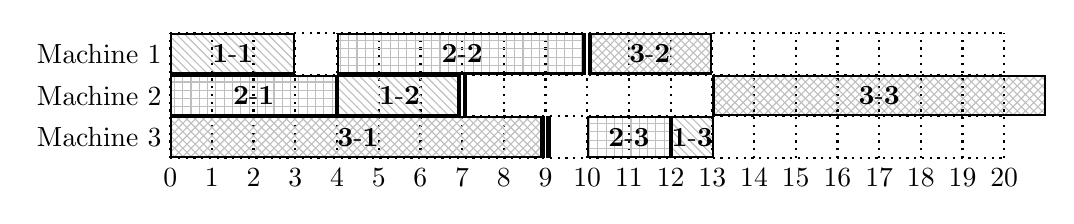
\begin{tikzpicture}[x=3.5ex,y=3.5ex,label distance=-1ex,thick]
\SetScales
\foreach \i in {1,...,3} {
  \node[label=left:Machine \i] at (0,3.5-\i) {};
}
\foreach \i in {0,...,20} {
  \draw[dotted] (\i,0) -- (\i,3) node [below] at (\i,0) {$\i$};
}
\foreach \i in {0,...,3} {
  \draw[dotted] (0,\i) -- (20,\i);
}
\node[minimum width=3\scaledx-0.05\scaledx,minimum height=1\scaledy-0.05\scaledy,inner sep=0,rectangle,draw,anchor=south west,pattern color=lightgray,pattern=north west lines] at (0,2) {\textbf{1}-\textbf{1}};
\node[minimum width=3\scaledx-0.05\scaledx,minimum height=1\scaledy-0.05\scaledy,inner sep=0,rectangle,draw,anchor=south west,pattern color=lightgray,pattern=crosshatch] at (10,2) {\textbf{3}-\textbf{2}};
\node[minimum width=6\scaledx-0.05\scaledx,minimum height=1\scaledy-0.05\scaledy,inner sep=0,rectangle,draw,anchor=south west,pattern color=lightgray,pattern=grid] at (4,2) {\textbf{2}-\textbf{2}};
\node[minimum width=4\scaledx-0.05\scaledx,minimum height=1\scaledy-0.05\scaledy,inner sep=0,rectangle,draw,anchor=south west,pattern color=lightgray,pattern=grid] at (0,1) {\textbf{2}-\textbf{1}};
\node[minimum width=3\scaledx-0.05\scaledx,minimum height=1\scaledy-0.05\scaledy,inner sep=0,rectangle,draw,anchor=south west,pattern color=lightgray,pattern=north west lines] at (4,1) {\textbf{1}-\textbf{2}};
\node[minimum width=8\scaledx-0.05\scaledx,minimum height=1\scaledy-0.05\scaledy,inner sep=0,rectangle,draw,anchor=south west,pattern color=lightgray,pattern=crosshatch] at (13,1) {\textbf{3}-\textbf{3}};
\node[minimum width=9\scaledx-0.05\scaledx,minimum height=1\scaledy-0.05\scaledy,inner sep=0,rectangle,draw,anchor=south west,pattern color=lightgray,pattern=crosshatch] at (0,0) {\textbf{3}-\textbf{1}};
\node[minimum width=1\scaledx-0.05\scaledx,minimum height=1\scaledy-0.05\scaledy,inner sep=0,rectangle,draw,anchor=south west,pattern color=lightgray,pattern=north west lines] at (12,0) {\textbf{1}-\textbf{3}};
\node[minimum width=2\scaledx-0.05\scaledx,minimum height=1\scaledy-0.05\scaledy,inner sep=0,rectangle,draw,anchor=south west,pattern color=lightgray,pattern=grid] at (10,0) {\textbf{2}-\textbf{3}};
\draw[ultra thick,double] (9,0) -- (9,1);
% \draw[ultra thick] (7,1) -- (9,1);
\draw[ultra thick,double] (7,1) -- (7,2);
% \draw[ultra thick] (7,2) -- (10,2);
\draw[ultra thick,double] (10,2) -- (10,3);
\end{tikzpicture}
\figspace
\caption{Decomposed schedule for example JSP instance\label{fig:decomposed}}% in Listing~\ref{prg:facts}\label{fig:schedule}}
\end{figure}

\section{Experiments}\label{sec:experiments}
This section will show the computational experiments that we conducted to test the performance of our proposed model. In order to evaluate our model, we performed several experiments on a set of benchmark instances with a different number of jobs and machines. The benchmark instances we considered are generated in 1993 by E. Taillard \cite{taillard1993benchmarks}, and the size of the problems variate starting from $6$ jobs and $6$ machines till $100$ jobs and $20$ machines. We have decided to focus on $3$ different sizes of the problem, which are $50$ jobs, $15$ machines, $50$ jobs and $20$ machines and $100$ jobs and $20$ machines. Our experiments had been conducted on a laptop with Intel(R) Core(TM) i7-8650U CPU @ 1.90GHz 2.11 GHz, 8th generation, and $16$ GB. We split the problem into a different number of TWs starting from $2$ - $10$ throughout each size of the instances we focused on to investigate the most appropriate number of TWs. We run the model with a fixed amount of time $1000$ seconds. We set this amount because we observed that increasing the time more did not provide better results, and when we reduced it, the results became worse. The next table shows the obtained results with solving $50 \times 15$.

\begin{comment}
\begin{table}[t]
    \caption{Results for three sizes of job shop scheduling instances with different numbers of time windows using static machine-based EST decomposition \label{tab:Table01}}%
%    \mbox{~}\hfill
%    \resizebox{0.8\textwidth}{!}{%
%    \begin{minipage}{\textwidth}
    \centering
    \begin{tabular}{l l r r r r r r r r r r}
    \hline
%       & {}        & \multicolumn{6}{c}{Group of Instances}  \\
    &  &  \multicolumn{10}{c}{Number of Time Windows} \\
    Instances & Comparison & 1 & 2 & 3 & 4 & 5 & 6 & 7 & 8 & 9 & 10 \\
                     
    \hline\\[-2.75mm]
    {50$\times$15}       & Makespan             & $3542.1$   & $3149.7$	     &  \boldmath{$3083.8$} & $3110.7$ & $3213.6$ & $3225.3$ & $3350.5$ & $3378.5$ & $3495.0$ & $3524.9$ \\
    & CPU(Sec)             & $1000.0$	& $1000.0$   & $1000.0$	 & $934.4$ & $615.5$  & $243.8$  & $146.7$ 	& $81.0$ & $45.6$ & $18.5$  \\
    & Interrupted Calls    & $1.0$	    & $2.0$      & $3.0$	& $3.6$  & $2.7$  & $1.0$  &  $0.6$  & $0.3$ & $0.1$ & $0.1$       \\[1.5mm]
    
    
    {50$\times$20}       & Makespan             & $3879.4$   & $3479.4$	      & $3290.5$  &  \boldmath{$3260.3$} &  $3355.5$ & $3414.8$ & $3540.3$  &  $3561.5$  & $3720.7$  & $3793.1$ \\
    & CPU(Sec)             & $1000.0$	    & $1000.0$	   & $1000.0$	  & $944.9$  & $583.4$  & $321.5$  &  $161.4$  & $54.9$  & $38.0$  & $33.3$     \\
    & Interrupted Calls    & $1.0$	    & $2.0$      & $3.0$	& $3.5$ & $2.5$  & $1.6$  & $0.9$  & $0.2$ & $0.2$  & $0.1$      \\[1.5mm]
    
    {100$\times$20}      & Makespan             & $46786.1$  &  $23977.5$  & $7201.5$ &  $6288.7$                & $6106.1$  &  \boldmath{$6031.9$} & $6094.1$ & $6053.1$ & $6095.9$  & $6234.0$  \\
    & CPU(Sec) & $1000.0$	    & $1000.0$	   & $1000.0$	   & $1000.0$	    & $1000.0$	& $1000.0$	& $1000.0$ & $1000.0$	    & $1000.0$	& $1000.0$            \\
    & Interrupted Calls    & $1.0$	    & $2.0$      & $3.0$	& $4.0$ & $5.0$  & $6.0$ & $7.0$ & $8.0$ & $8.2$ & $7.9$      \\[1.5mm]

                     
                     
    \\[-2.75mm]
    \hline
    \end{tabular}
   % }
%    \end{minipage}
% }
%    \hfill\hfill\mbox{~}
\end{table}}

\end{comment}

\begin{table}[t]
    \caption{Results for three sizes of job shop scheduling instances with different numbers of time windows using static machine-based EST decomposition \label{tab:Table01}}%
%    \mbox{~}\hfill
%    \resizebox{0.8\textwidth}{!}{%
%    \begin{minipage}{\textwidth}
    \centering
    \begin{tabular}{l l r r r r r r r}
    \hline
%       & {}        & \multicolumn{6}{c}{Group of Instances}  \\
    &  &  \multicolumn{7}{c}{Number of Time Windows} \\
    Instances & Comparison & 1 & 2 & 3 & 4 & 5 & 6 & 10 \\
                     
    \hline\\[-2.75mm]
    
    {50$\times$15}       & Makespan             & $3542.1$   & $3149.7$	     &  \boldmath{$3083.8$} & $3110.7$ & $3213.6$ & $3225.3$ & $3524.9$ \\
    & CPU(Sec)             & $1000.0$	& $1000.0$   & $1000.0$	 & $934.4$ & $615.5$  & $243.8$  & $18.5$  \\
    & Interrupted Calls    & $1.0$	    & $2.0$      & $3.0$	& $3.6$  & $2.7$  & $1.0$  & $0.1$       \\[1.5mm]
    

    {50$\times$20}       & Makespan             & $3879.4$   & $3479.4$	      & $3290.5$  &  \boldmath{$3260.3$} &  $3355.5$ & $3414.8$ & $3793.1$ \\
    & CPU(Sec)             & $1000.0$	    & $1000.0$	   & $1000.0$	  & $944.9$  & $583.4$  & $321.5$   & $33.3$     \\
    & Interrupted Calls    & $1.0$	    & $2.0$      & $3.0$	& $3.5$ & $2.5$  & $1.6$  & $0.1$      \\[1.5mm]

    {100$\times$20}      & Makespan             & $46786.1$  &  $26210.4$  & $7201.5$ &  $6288.7$                & $6106.1$  &  \boldmath{$6031.9$}   & $6234.0$  \\
    & CPU(Sec) & $1000.0$	    & $1000.0$	   & $1000.0$	   & $1000.0$	    & $1000.0$	& $1000.0$	& $861.8$            \\
    & Interrupted Calls    & $1.0$	    & $2.0$      & $3.0$	& $4.0$ & $5.0$  & $6.0$ & $7.9$      \\[1.5mm]
                     
    \\[-2.75mm]
    \hline
    \end{tabular}
   % }
%    \end{minipage}
% }
%    \hfill\hfill\mbox{~}
\end{table}

Table \ref{tab:Table01} shows the results of solving the mentioned different sizes before with a machine-based EST decomposition method.
The columns represent how many windows split the original problem where TW $1$ refers that the problem is not decomposed. The results of $7, 8$ and $9$ TWs have not been presented because they have not changed the tendency of the results. Every three rows show the average makespan, running time and the number of interrupted calls of a particular size of the instances. We run the model with a fixed amount of time $1000$ seconds divided by TWs for each window. It is observed that increasing the timeout does not provide better results, and when we decrease it, the results become worse. The best-obtained average makespan for the $50\times15$ instances is $3083.8$ with $3$ TWs where the number of operations assigned to each window is $250$. In addition, increasing the TWs supported the optimizer to reach an optimal of a sub-problem, as the number of operations assigned to a TW decreased. Therefore, The average running time for 10 TWs is $18.5$ seconds. However, the average makespan is getting worse.\\

The number of windows with the best obtained average makespan $3260.3$ for scheduling $50\times20$ is $4$ with an average timeout of $944.9$. We observe that assigning $250$ operations to each window leads to getting the best average makespan for the first two sets. For the $100\times20$ set, we got an average makespan of $6031.9$ with $6$ TWs and $1000$ seconds timeout, where the optimizer could not reach a sub-optimal for any TW. 

\begin{table}[t]
    \caption{Comparing different static/dynamic decomposition strategies \label{tab:Table02}}%
%    \mbox{~}\hfill
%    \resizebox{0.8\textwidth}{!}{%
%    \begin{minipage}{\textwidth}
    \centering
    \begin{tabular}{c c c c c c c c c c}
    \hline
  
\multirow{2}*{Strategy} & \multicolumn{3}{c}{50$\times$15} & \multicolumn{3}{c}{50$\times$20} & \multicolumn{3}{c}{100$\times$20}\\
    & Makespan & Time & IC & Makespan & Time & IC & Makespan & Time & IC \\
    \hline\\[-2.75mm]
    M-Based EST (S)             & $3083.8$  & $1000.0$   & $3.0$	& \boldmath{$3260.3$}      & $944.9$ & $3.5$ & $6031.9$ & $1000.0$ & $6.0$\\
    [1.5mm]

    T-based EST (S)            & $3524.8$ & $1000.0$   & $2.0$	   & $3540.8$      & $1000.0$ & $2.0$ & $6964.4$ & $1000.0$ & $4.0$\\ 
    [1.5mm]
    
    M-based MTWR (S)        & \boldmath{$3060.3$}  & $1000.0$   & $3.0$	& $3287.9$      & $986.1$ & $3.9$ & \boldmath{$5948.6$} & $1000.0$ & $7.0$\\ 
    [1.5mm]
    
    T-based MTWR (S)            & $3456.2$  & $1000.0$   & $2.0$	& $3561.0$      & $1000.0$ & $2.0$ & $7149.6$ & $1000.0$ & $4.0$\\ 
    [1.5mm]

    M-based EST (D)            & $3098.4$  & $1000.0$   & $3.0$	& $3309.5$     & $1000.0$ & $3.3$ & $6115.1$ & $1000.0$ & $6.9$\\ 
    [1.5mm]

    \\[-2.75mm]
    \hline
    
    
    
    \end{tabular}
   % }
%    \end{minipage}
% }
%    \hfill\hfill\mbox{~}
\end{table}



\begin{table}[t]
    \caption{Comparing results of best decomposition strategy with/without dompression and overlapping \label{tab:Table03}}%
%    \mbox{~}\hfill
%    \resizebox{0.8\textwidth}{!}{%
%    \begin{minipage}{\textwidth}
    \centering
    \begin{tabular}{c c c c c c c c c c}

    \hline
    \multicolumn{10}{c}{\textbf{Without Compressing Time Windows}}\\        
\multirow{2}*{Overlap} & \multicolumn{3}{c}{50$\times$15} & \multicolumn{3}{c}{50$\times$20} & \multicolumn{3}{c}{100$\times$20}\\
    & Makespan & CPU(Sec) & IC & Makespan & CPU(Sec) & IC & Makespan & CPU(Sec) & IC \\
    \hline\\[-2.75mm]
    0\%              & $3083.8$  & $1000.0$   & $3.0$	& $3260.3$      & $944.9$ & $3.5$ & $6031.9$ & $1000.0$ & $6.0$\\
    [1.5mm]
                     
    10\%             & $3050.0$  & $1000.0$   & $3.0$	& \boldmath{$3194.9$}     & $1000.0$ & $4.0$ & $5979.9$ & $1000.0$ & $6.0$\\ 
    
    20\%             & \boldmath{$3046.0$} & $1000.0$   & $3.0$	   & $3200.6$      & $1000.0$ & $4.0$ & \boldmath{$5954.3$} & $1000.0$ & $6.0$\\ 
    
    30\%             & $3051.2$  & $1000.0$   & $3.0$	& $3451.8$      & $1000.0$ & $4.0$ & $6933.3$ & $1000.0$ & $6.0$\\ 
                     [1.5mm]
                     
    \\[-2.75mm]
    
    \multicolumn{10}{c}{\textbf{Compressing Time Windows}}\\
    \hline
    \multirow{2}*{Overlap} & \multicolumn{3}{c}{50$\times$15} & \multicolumn{3}{c}{50$\times$20} & \multicolumn{3}{c}{100$\times$20}\\
    & Makespan & CPU(Sec) & IC & Makespan & CPU(Sec) & IC & Makespan & CPU(Sec) & IC \\
    \hline\\[-2.75mm]
    0\%              & $3013.3$  & $572.3$   & $3.7$	   & $3186.8$      & $540.8$ & $3.3$ & $5713.0$ & $589.2$ & $8.6$\\
    [1.5mm]
                     
    10\%             & $2970.2$  & $600.0$   & $4.0$	   & $3149.8$      & $600.0$ & $4.0$ & $5656.0$ & $600.0$ & $9.0$\\ 
    
    20\%             & $2952.2$  & $600.0$   & $4.0$	   & \boldmath{$3147.7$}      & $600.0$ & $4.0$ & \boldmath{$5619.2$} & $600.0$ & $9.0$\\ 
    
    30\%             & \boldmath{$2943.1$}  & $600.0$   & $4.0$	   & $3162.2$      & $600.0$ & $4.0$ & $5857.0$ & $600.0$ & $9.0$\\ 
                     [1.5mm]
    \hline
    \end{tabular}
   % }
%    \end{minipage}
% }
%    \hfill\hfill\mbox{~}
\end{table}

Table \ref{tab:Table02} demonstrates the results of the four static decomposition strategies and the machine-based MTWR with the dynamic assignment. Every three sub-columns have illustrated the results of a set of the benchmark instances and each row refers to a decomposition strategy with static (S) or dynamic (D) assignment. The results of this table conclude that the most effective decomposition strategies are machine-based regardless of whether the operations are ordered based on EST or MTWR; however, the dynamic assignment has no positive effect than the static. %The best average makespan of $50\times15$ and $100\times20$ are  $3060.3$, and $5948.6$.
We applied the overlap between the windows to repair the mistakes generated by the decomposition; in addition, we compressed each optimized window to ensure that all the operations had been started as early as possible. Table \ref{tab:Table03} summarizes the results with/without the compression and the overlap. The first column refers to the overlap percentage where $0\%$ means no overlap between TWs. Every three columns have presented the results of a particular set of instances. We applied the overlap and compression with the solutions of the number of windows, which provided a better average makespan using a machine-based EST strategy. In the non-compression part, the overlap has improved the results slightly through the different sizes where $10\%$ and $20\%$ of overlap provided the best results. However, the compression has shown a significant improvement wrt the running time and the average makespan, especially for the $100\times20$ set. The compression demonstrated effectiveness as it minimized the average makespan and decreased the running time compared to the model without compression. Therefore, the overlap and compression have improved the makespan results by $4.5\%, 3.4\%$ and $6.8\%$ and the running time by $40\%$.

\section{Conclusions}\label{sec:conclusions}
In this work, different decomposition strategies have been proposed for solving the Job-shop Scheduling Problem (JSP) using a multi-shot Answer Set Programming with Difference Logic constraints to handle the decomposition approach and the problem constraints. The proposed model split the problem into sub-problems using different decomposition strategies and then optimized each separately while minimizing the Makespan. The proposed model has been developed to improve the performance by applying the overlap between TWs to fix the decomposition mistakes. In addition, the compression of each window is to fulfill the gaps that occurred during the optimization process. We tested our model on a set of benchmark instances and the experiments have shown that i) considering the bottleneck machines during the decomposition process is effective, ii) The overlap between TWs improves the solution quality, and iii) the compression of TWs is super practical, as it aided the proposed model to obtain better solutions in less computational time. Our work can be extended by linking the optimization model with a simulator that considers more realistic factors such as machine breakdowns, new job arrivals and order cancellations.

%
% ---- Bibliography ----
%
% BibTeX users should specify bibliography style 'splncs04'.
% References will then be sorted and formatted in the correct style.
%
% \bibliographystyle{splncs04}
% \bibliography{mybibliography}
%
\bibliographystyle{tlplike} % \bibliographystyle{splncs04}
\bibliography{Ref}

\end{document}
